\section{Entwurf der Bedienoberfläche}
\label{sec:substitution}
%Marcus

Im Rahmen der Kursarbeit gilt es, die Entwurfsgrundsätze von Bedienoberflächen kennenzulernen, auf das eigene Softwareprojekt anzuwenden und eine Auswahl aus unterschiedlichen Möglichkeiten zur Informationsdarstellung basierend auf Vor- und Nachteilen zu treffen. Dazu wird der Vorgang des Oberflächenentwurfs als iterativer Prozess aufgefasst, in welchem das Team als Designer und Entwickler die Zielgruppenanalyse als Handlungsbasis für den Entwurf von Mockups interpretiert. Dadurch bilden die Entwürfe der Bedienoberfläche ein direktes Resultat der Beobachtung der Benutzer, ihrer Aufaben und Intentionen \cite{La05}. Für Equaly bedeutete dies den Entwurf einer Weboberfläche für Texteingabe und Anzeige des gegenderten Textresultats. Die Diversität der ausgemachten Zielgruppen und die geplante Platzierung von Equaly als Hilfsmittel führten zu dem Entschluss, die Oberfläche möglichst übersichtlich und einfach aufzubauen. Für den Gendering-Prozess bildet der nutzerseitig eingegebene Text die Handlungsgrundlage. Entsprechend sollte die Oberfläche um die Kernkompetenz der intuitiven Ein- und Ausgabe von Text aufgebaut werden. Der aus dieser Phase favorisierte Mockup ist in \ref{fig:mockup} dargestellt.

\begin{figure}[!th]
\centering
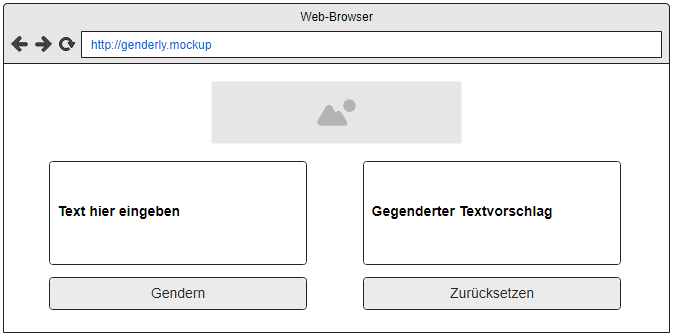
\includegraphics[width=8cm]{Resources/Mockup.PNG}
\caption{Favorisierter Mockup für die Weboberfläche von Equaly}
\label{fig:mockup}
\end{figure}

Neben der Anordnung der Elemente wurde auch die farbliche Gestaltung entworfen. Es galt, Farben derartig einzusetzen, dass die Oberfläche einen Wiedererkennungswert und Aufmerksamkeit bei den Zielgruppen erreichen würde. Eine erarbeitete Farbgebung richtete sich danach, wie die UN für das 5. Ziel für die nachhaltige Entwicklung gestaltete. Die entsprechend orange Gestaltung sollte Aufmerksamkeit erregen, gleichzeitig aber auch die positive Motivation hinter Equaly unterstreichen.